\documentclass[border=4pt]{standalone}

\usepackage{amsmath}
\usepackage{tikz}
\usepackage{mathdots}
\usepackage{yhmath}
\usepackage{cancel}
\usepackage{color}
\usepackage{siunitx}
\usepackage{array}
\usepackage{multirow}
\usepackage{amssymb}
\usepackage{gensymb}
\usepackage{tabularx}
\usepackage{booktabs}
\usetikzlibrary{fadings}
\usetikzlibrary{patterns}


\begin{document}
 

\tikzset{every picture/.style={line width=0.75pt}} %set default line width to 0.75pt        

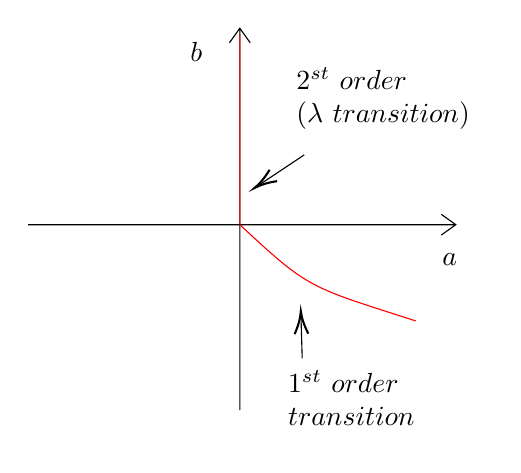
\begin{tikzpicture}[x=0.75pt,y=0.75pt,yscale=-1,xscale=1]
%uncomment if require: \path (0,300); %set diagram left start at 0, and has height of 300

%Shape: Axis 2D [id:dp6713916455701754] 
\draw  (127,152.66) -- (333,152.66)(228.95,58) -- (228.95,242) (326,147.66) -- (333,152.66) -- (326,157.66) (223.95,65) -- (228.95,58) -- (233.95,65)  ;
%Straight Lines [id:da8777392314880006] 
\draw [color={rgb, 255:red, 255; green, 0; blue, 0 }  ,draw opacity=1 ]   (229,61) -- (228.95,152.66) ;


%Curve Lines [id:da5568798247772362] 
\draw [color={rgb, 255:red, 255; green, 0; blue, 0 }  ,draw opacity=1 ]   (228.95,152.66) .. controls (262.33,183.67) and (261.67,182.33) .. (313.67,199) ;


%Straight Lines [id:da31539843136283485] 
\draw    (259,217) -- (258.39,196.33) ;
\draw [shift={(258.33,194.33)}, rotate = 448.32] [color={rgb, 255:red, 0; green, 0; blue, 0 }  ][line width=0.75]    (10.93,-3.29) .. controls (6.95,-1.4) and (3.31,-0.3) .. (0,0) .. controls (3.31,0.3) and (6.95,1.4) .. (10.93,3.29)   ;

%Straight Lines [id:da14322319381180693] 
\draw    (260,119) -- (237.66,133.89) ;
\draw [shift={(236,135)}, rotate = 326.31] [color={rgb, 255:red, 0; green, 0; blue, 0 }  ][line width=0.75]    (10.93,-3.29) .. controls (6.95,-1.4) and (3.31,-0.3) .. (0,0) .. controls (3.31,0.3) and (6.95,1.4) .. (10.93,3.29)   ;


% Text Node
\draw (208,69.33) node    {$b$};
% Text Node
\draw (330,169.67) node    {$a$};
% Text Node
\draw (282.67,238.33) node    {$ \begin{array}{l}
1^{st} \ order\ \\
transition
\end{array}$};
% Text Node
\draw (298,92.33) node    {$ \begin{array}{l}
2^{st} \ order\ \\
( \lambda \ transition)
\end{array}$};


\end{tikzpicture}

\end{document}
